\documentclass[%14pt,
  handout, % no transitions
  ]{beamer}

\usepackage{ifluatex}

\ifluatex
  \usepackage{fontspec}
\fi

\usepackage[%english,
            %latin,
            spanish, es-minimal, es-nolists, es-nolayout, es-noshorthands, es-noquoting, es-uppernames, es-tabla
            ]{babel} % el último es el principal

\ifluatex
% LuaLaTeX --------------------
\defaultfontfeatures{Ligatures=TeX, Scale=MatchLowercase}
\setmainfont[Ligatures=Common,
Numbers=OldStyle,
% SmallCapsFeatures = {LetterSpace=5.0},
% BoldFont = {LinLibertineOZ},
% SmallCapsFeatures={Renderer=Basic},
]{Libertinus Serif}
% \setsansfont{Libertinus Sans}
\setmonofont[Scale=MatchLowercase]{DejaVu Sans Mono}
% \setmonofont[Scale=MatchLowercase]{Libertinus Mono}
% \setmonofont[Scale=MatchLowercase}]{Fira Code}
\else
% PDFLaTeX ---------------------
\usepackage[T1]{fontenc}
\usepackage[utf8]{inputenc}
% \usepackage[osf]{libertinus}
% \usepackage[osf]{fbb}
% \usepackage[osf]{ETbb}
% \usepackage[osf]{coelacanth}
% \usepackage[p,osf]{baskervillef}
% \usepackage{imfellEnglish}
% \usepackage[osf]{Alegreya} %% Option 'black' gives heavier bold face 
\usepackage[oldstylenums, nott, largesmallcaps]{kpfonts}
% \usepackage[osf]{cochineal}
% \usepackage[osf]{CormorantGaramond}
% \usepackage[osf]{ebgaramond}
% \usepackage[osf]{garamondx}
% \usepackage[osf]{Baskervaldx}
% \usepackage[osf]{newtxtext} % Times
% \usepackage{cfr-lm} % Latin Modern with OSF
% \usepackage[osf]{noto}
% \usepackage{lmodern} % Latin Modern
% \usepackage[scaled=0.95]{inconsolata}
\usepackage[scaled=0.7]{DejaVuSansMono}
\usepackage[scaled=0.9]{atkinson}
% \usepackage[scaled=0.9]{roboto} 
% \usepackage{josefin}
% \usepackage[scaled=0.9]{FiraSans}
% \usepackage{AlegreyaSans}
% \usepackage[scaled=0.8]{DejaVuSans}
\fi

% \usetheme{Nivaca}
\usetheme{Leuven}

\usepackage{latexcolors}

\newcommand{\Rojo}{\color[HTML]{8B0000}}
\newcommand*{\rojo}[1]{\textcolor[HTML]{8B0000}{#1}}
\newcommand*{\rojoit}[1]{\textit{\textcolor[HTML]{8B0000}{#1}}}
\newcommand{\Azul}{\color{bluenivaca}}
\newcommand*{\azul}[1]{\textcolor{bluenivaca}{#1}}
\newcommand{\Verde}{\color{seagreen}}
\newcommand*{\verde}[1]{\textcolor{seagreen}{#1}}
\newcommand{\Amarillo}{\color{goldenpoppy}}
\newcommand*{\amarillo}[1]{\textcolor{goldenpoppy}{#1}}
\newcommand{\Morado}{\color{byzantium}}
\newcommand*{\morado}[1]{\textcolor{byzantium}{#1}}
\newcommand{\Naranja}{\color{orange}}
\newcommand*{\naranja}[1]{\textcolor{orange}{#1}}

\usepackage[autostyle=false, style=british]{csquotes}


\usepackage{xparse}
\usepackage{graphicx}
\usepackage{tikz}

\NewDocumentCommand \FrameImg { o m }
{%
\begingroup
\setbeamercolor{background canvas}{bg=white}%
\setbeamertemplate{navigation symbols}{}%
\begin{frame}[plain]%
  \centering%
  \IfValueTF {#1}
  {\includegraphics[width=\textwidth, height=.93\textheight, keepaspectratio]{img/#2}\\\Azul\footnotesize#1}%
  {\includegraphics[width=\textwidth, height=\textheight, keepaspectratio]{img/#2}}
\end{frame}%
\endgroup%
}


\newcommand*{\elipsis}{\,.\,.\,.\,}
\newcommand*{\elipsisb}{\textup{[\elipsis]}}
\newcommand*{\TEI}{\textsc{tei}}
\newcommand*{\XML}{\textsc{xml}}

\usepackage{minted}

\definecolor{Link}{HTML}{408080}
\usepackage{hyperref}
\hypersetup{
  colorlinks=true,
  linkcolor=Link,
  filecolor=Link,
  citecolor=black,      
  urlcolor=Link,
}
\urlstyle{tt}
% ====================================================



\title{Herramientas Digitales}
\subtitle{Introducción a \TEI\ 1}

\author{Nicolás Vaughan}
\institute[UA]
{\footnotesize
Universidad de los Andes \\
\medskip
\texttt{n.vaughan@uniandes.edu.co}
}


% \def\mydate{\today}
\def\mydate{2023-05-12}
\date[\tiny\mydate]{\scriptsize\mydate}

\begin{document}

\begin{frame}
  \titlepage
\end{frame}

% \begin{frame}
% \frametitle{Contenido}
% \tableofcontents
% \end{frame}


\begin{frame}
  \frametitle{Análogo / digital}
  
  {\large\Azul\textbf{¿Qué significa \enquote{digitalizar}?}}

  \bigskip

  \rojo{1.} \rojoit{Escanear} --- transformar una imagen analógica a un archivo digital gráfico (\texttt{.png}, \texttt{.tiff}, \texttt{.jpeg}, etc).

  \begin{center}
    
\includegraphics[width=0.5\textwidth]{img/scanning.png}
  \end{center}

\end{frame}


\begin{frame}
  \frametitle{Análogo / digital}
  
  {\large\Azul\textbf{¿Qué significa \enquote{digitalizar}?}}

  \bigskip

  \rojo{2.} \rojoit{OCR} --- reconocimiento óptico de caracteres

  \begin{center}
    
\includegraphics[width=0.4\textwidth]{img/image.png} %
    \quad%
    \raisebox{2cm}{{\Rojo\Huge$\Rightarrow$}}
    \quad%
    
\includegraphics[width=0.4\textwidth]{img/text.png} %
    
  \end{center}

\end{frame}



\begin{frame}
  \frametitle{Análogo / digital}
  
  {\large\Azul\textbf{¿Qué significa \enquote{digitalizar}?}}

  \bigskip

  \rojo{3.} \rojoit{Marcado / etiquetado (\textit{tagging})} --- darle \textit{significado} al texto

  \begin{center}
    \begin{itemize}
      \item representacional o gráfico (\textsc{html}, \LaTeX, Troff, \textsc{xsl-fo}, etc.)
      \item semántico:
        \begin{itemize}
          \item análisis y crítica textual
          \item lingüístico
          \item análisis cualitativo (qdap, \textsc{atlas}.ti, NVivo, etc.)
          \item \dots
        \end{itemize}
    \end{itemize}
    
  \end{center}

\end{frame}



\FrameImg[Codificación categorías en \textsc{atlas}.ti]{atlasti.png}


% \begin{frame}[fragile]
%   \frametitle{Marcado representacional en \textsc{html}}

%   \begin{minipage}[c]{0.5\linewidth}
% \scriptsize
% \begin{minted}{html}
  
% <!-- ... -->  
% <h1>Este es un título de nivel 1</h1>
% <em>Este texto aparece en cursivas</em>
% y <strong>este en negritas.</strong>

% <br />

% Una lista de viñetas:
% <ul>
%   <li>un ítem</li>
%   <li>otro ítem</li>
%   <li>otro ítem</li>
% </ul>

% <br />

% <span style="color: red">
%   Este texto va en rojo.
% </span>
% <!-- ... --> 
%     \end{minted}
%   \end{minipage}%
%   \begin{minipage}[t][\textwidth][t]{0.5\linewidth}
%     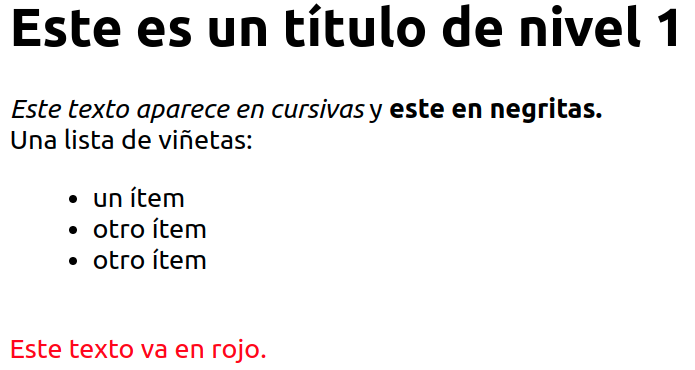
\includegraphics[width=\textwidth]{img/html.png}
%   \end{minipage}
    
% \end{frame}


\begin{frame}
  \frametitle{El marcado: ¿para qué?}
  \begin{itemize}
    \item Para poder \rojoit{representar} correctamente su contenido (en una pantalla, en un papel, etc.)
    \item Para poder \rojoit{interpretar} correctamente su contenido
  \end{itemize}

  \bigskip

  En cualquier caso, es importante que el marcado sea \textit{procesable por el computador} (\textit{machine-readable}).
  
\end{frame}



\begin{frame}[fragile]
  \frametitle{Marcado representacional en \textsc{html}}

  \begin{minipage}[c]{0.5\linewidth}
\scriptsize
\begin{verbatim}
  
<!-- ... -->  
<h1>Este es un título de nivel 1</h1>
<em>Este texto aparece en cursivas</em>
y <strong>este en negritas.</strong>

<br />

Una lista de viñetas:
<ul>
  <li>un ítem</li>
  <li>otro ítem</li>
  <li>otro ítem</li>
</ul>

<br />

<span style="color: red">
  Este texto va en rojo.
</span>
<!-- ... --> 
    \end{verbatim}
  \end{minipage}%
  \begin{minipage}[t][\textwidth][t]{0.5\linewidth}
    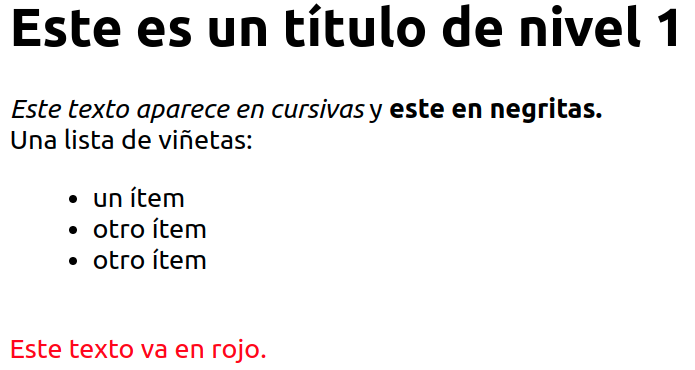
\includegraphics[width=\textwidth]{img/html.png}
  \end{minipage}
    
\end{frame}


\begin{frame}[fragile]
  \frametitle{Marcado semántico en \TEI}

  \begin{minted}{xml}
<!-- ... --> 
  <persName>Moctezuma Xocoyotzin</persName> nació en <date>1466</date>, 
  y murió el <date>29 de junio en 1520</date>
  en <placeName>Tenochtitlan</placeName>, <placeName>México</placeName>.
<!-- ... --> 
\end{minted}
  
\end{frame}


\begin{frame}
  \frametitle{¿Qué es \TEI?}

\large\centering
  
\rojo{\TEI\ ({\small\textit{Text Encoding Initiative}})} es una implementación del lenguaje de marcado \azul{\XML} diseñada para codificar o marcar semánticamente textos de diversas índoles.

\bigskip

Por su parte, \azul{\XML\ ({\small\textit{Extensible Markup Language}})} es un lenguaje de marcado general usado para codificar todo tipo de información.
\end{frame}


\begin{frame}[fragile]
  \frametitle{Ejemplo de un documento \XML}
\scriptsize
  \begin{minted}{xml}
<?xml version="1.0"?>
<catalog>
  <book id="bk101">
    <author>Gambardella, Matthew</author>
    <title>XML Developer's Guide</title>
    <genre>Computer</genre>
    <price>44.95</price>
    <publish_date>2000-10-01</publish_date>
    <description>An in-depth look at creating applications 
      with XML.</description>
  </book>
  <book id="bk102">
    <author>Ralls, Kim</author>
    <title>Midnight Rain</title>
    <genre>Fantasy</genre>
    <price>5.95</price>
    <publish_date>2000-12-16</publish_date>
    <description>A former architect battles corporate zombies, 
      an evil sorceress, and her own childhood to become queen 
      of the world.</description>
  </book>
</catalog>
  \end{minted}
\end{frame}


\begin{frame}[fragile]
  \frametitle{\XML: algunas definiciones}
  \begin{enumerate}
    \item \rojoit{Elementos} --- son los pilares estructurales de un documento \XML.

      Se componen de:
      \begin{itemize}
        \item una \textit{etiqueta de apertura}
        \item una \textit{etiqueta de cierre}
        \item un \textit{contenido} (que puede ser otros elementos, texto o nada)
        \item y opcionalmente unos \textit{atributos} con sus \textit{valores} correspondientes.
      \end{itemize}
      Ejemplos:

      \begin{itemize}
        \item \mintinline{xml}{<persName>Moctezuma Xocoyotzin</persName>}
        \item \mintinline{xml}{<date when="2022-12-31">31 de diciembre de 2022</persName>}
        \item \mintinline{xml}{<date when="2022-12-31" calendar="juliano">diciembre 31</persName>}
        \item
\begin{minted}{xml}
<persName>
  <forename>William</forename>
  <surname>Shakespeare</surname>
</persName>
\end{minted}
          
        \item \mintinline{xml}{<lb></lb>} (o equivalentemente \mintinline{xml}{<lb/>})
        \item \mintinline{xml}{<lb n="3"></lb>} (o equivalentemente \mintinline{xml}{<lb n="3"/>})
      \end{itemize}
  \end{enumerate}
\end{frame}

\begin{frame}[fragile]
  \frametitle{\XML: algunas definiciones}
  \begin{enumerate}
    \setcounter{enumi}{1}
    \item \rojoit{Entidades}: \XML\ contiene cinco caracteres que no pueden usarse literalmente sino solo por medio de una referencia:

      \begin{center}
        \begin{tabular}{ll}
          \texttt{\&quot} & \texttt{"} \\
          \texttt{\&amp}  & \texttt{\&} \\
          \texttt{\&apos} & \texttt{'} \\
          \texttt{\&lt}   & \texttt{<} \\
          \texttt{\&gt}   & \texttt{>} \\
        \end{tabular}
      \end{center}
      
    \item \rojoit{Padres, hijos, ancestros y descendientes}: si un elemento contiene otro elemento, el primero se denomina el \textit{padre}, y el segundo el \textit{hijo}. Un elemento puede tener muchos \textit{ancestros} y muchos \textit{descendientes}.
      
    \item \rojoit{Declaración}: está al principio de un documento \XML, identificándolo como tal: \mintinline{xml}|<?xml version="1.0" encoding="UTF-8"?>|
  \end{enumerate}
\end{frame}



\begin{frame}[fragile]
  \frametitle{\XML: algunas definiciones}
  \begin{enumerate}
    \setcounter{enumi}{4}
    \item \rojoit{Instrucciones de procesamiento}: van debajo de la declaración \XML\ y especifican el modo como el documento debe ser validado semánticamente o procesado. Empiezan con \verb|<?| y terminan con \verb|?>|.

      \bigskip

      Por ejemplo, para validar un documento \XML\ con el esquema de validación de \TEI\ (más exactamente, el de \TEI-all), debemos incluir lo siguiente:

\begin{minted}{xml}
<?xml-model href="http://www.tei-c.org/release/xml/tei/custom/schema/
  relaxng/tei_all.rng" type="application/xml"
  schematypens="http://relaxng.org/ns/structure/1.0"?>
<?xml-model href="http://www.tei-c.org/release/xml/tei/custom/schema/
  relaxng/tei_all.rng" type="application/xml"
  schematypens="http://purl.oclc.org/dsdl/schematron"?>
\end{minted}
  \end{enumerate}
\end{frame}


\begin{frame}[fragile]
  \frametitle{Reglas fundamentales de un documento \XML}
  \begin{enumerate}
    \item Todo documento \XML\ debe tener un único elemento raíz.
      \scriptsize
    \item[] \verde{\textsc{correcto}:}
\begin{minted}{xml}
<biblio>
  <libro>
    <título>Cien años de soledad</título>
    <autor>Gabriel García Márquez</autor>
  </libro>
  <libro>
    <título>El coronel no tiene quien le escriba</título>
    <autor>Gabriel García Márquez</autor>
  </libro>
</biblio>
\end{minted}

    \item[] \rojo{\textsc{incorrecto}:}
       \scriptsize
\begin{minted}{xml}
<libro>
  <título>Cien años de soledad</título>
  <autor>Gabriel García Márquez</autor>
</libro>
<libro>
  <título>El coronel no tiene quien le escriba</título>
  <autor>Gabriel García Márquez</autor>
</libro>
\end{minted}
  \end{enumerate}
\end{frame}

\begin{frame}[fragile]
  \frametitle{Reglas fundamentales de un documento \XML}
  \begin{enumerate}
      \setcounter{enumi}{1}  
    \item Todo elemento empieza con una etiqueta de apertura y cierra con una etiqueta de cierre.

    \item[] \verde{\textsc{correcto}:}
\begin{minted}{xml}
<p>
  <title>Cien años de soledad</title>
  <author>Gabriel García Márquez</author>
</p>
\end{minted}

    \item[] \rojo{\textsc{incorrecto}:}
\begin{minted}{xml}
<p>
  <title>Cien años de soledad
  <author>Gabriel García Márquez</author>
</p>
\end{minted}
      
  \end{enumerate}
\end{frame}

\begin{frame}[fragile]
  \frametitle{Reglas fundamentales de un documento \XML}
  \begin{enumerate}
      \setcounter{enumi}{2}
    \item Todo elemento debe ser apropiadamente anidado.

      \medskip

      \begin{minipage}{0.4\linewidth}
      \verde{\textsc{correcto}:}
\begin{minted}{xml}
<p>
  <q>Esta es una cita</q>
</p>

\end{minted}        
    \end{minipage}%
      \hfill%
      \begin{minipage}{0.5\linewidth}
   \rojo{\textsc{incorrecto}:}
\begin{minted}{xml}
<p>
  <q>Esta es una cita</p>
</q>

\end{minted}
      \end{minipage}%
      
    \item Los nombres de los elementos no pueden empezar con \enquote{xml}, números o puntuación (excepto \enquote{\_}).

      \medskip
      
      \begin{minipage}{0.4\linewidth}
      \verde{\textsc{correcto}:}
\begin{minted}{xml}
<author>
<_author>
\end{minted}        
    \end{minipage}%
      \hfill%
      \begin{minipage}{0.5\linewidth}
   \rojo{\textsc{incorrecto}:}
\begin{minted}{java}
<01_author>
<"author">
\end{minted}
      \end{minipage}%
  \end{enumerate}
\end{frame}






\begin{frame}[fragile]
  \frametitle{Reglas fundamentales de un documento \XML}
  \begin{enumerate}
      \setcounter{enumi}{4}
    \item Los espacios en blanco (caracteres de espacio, de tabulador y de salto de línea) \textit{no} son significativos. \XML\ suele tragarse los espacios múltiples.

      \medskip
      
    \item[] Esto:
\begin{minted}{xml}
<p>
  <title>
    Cien       años        de      soledad
  </title>
                    </p>
\end{minted}

      \bigskip

    \item[] es equivalente a esto:
\small
\begin{minted}{xml}
<p><title>Cien años de soledad</title></p>
\end{minted}      

      
  \end{enumerate}
\end{frame}


\begin{frame}[fragile]
  \frametitle{Validez sintáctica y semántica}
  \begin{itemize}
    \item Un documento \XML\ es \rojoit{sintácticamente} válido si cumple con las reglas anteriores.
    \item Un documento \XML\ es \rojoit{semánticamente} válido si cumple con las reglas de un \textit{esquema de validación}.
      
      \begin{itemize}
        \item Para nuestro caso, un documento \azul{\XML-\TEI} es semánticamente válido si cumple con las reglas prescritas por el consorcio \TEI\ sobre el tipo de elementos (y sus atributos) y las relaciones existentes entre ellos.
        \item Por ejemplo, que la raíz de todo documento debe ser el elemento \mintinline{xml}|<TEI xmlns="http://www.tei-c.org/ns/1.0">|.
        \item Y que dicho elemento debe tener obligatoriamente dos elementos hijos: \mintinline{xml}|<teiHeader>| y \mintinline{xml}|<body>|.
        \item Y que el elemento \mintinline{xml}|<p>| puede tener algunos atributos (e.g. \texttt{ana, cert, copyOf,} etc.), pero no puede tener otros (e.g. \texttt{type}).
        \item Y así sucesivamente.
      \end{itemize}
      
    \item[] \url{https://www.tei-c.org/release/doc/tei-p5-doc/en/html/index.html}
  \end{itemize}
\end{frame}


\begin{frame}
  \frametitle{El flujo de trabajo}
  \begin{enumerate}
    \item La transcripción del documento (que puede ser manuscrito o impreso, en cuyo caso se puede usar \textsc{ocr})
    \item Codificación en \TEI
    \item Transformación del documento \TEI\ resultante para su procesamiento, análisis, reutilización, etc. 
    \item[] Por ejemplo:
      \begin{itemize}
        \item \TEI\ $+$ \href{https://www.w3.org/TR/xslt/}{\textsc{xslt}} $\rightarrow$ \XML
        \item \TEI\ $+$ \textsc{xslt} $\rightarrow$ \textsc{(x)html}
        \item \TEI\ $+$ \textsc{xslt} $\rightarrow$ texto plano
        \item \TEI\ $+$ \textsc{xslt} $\rightarrow$ \href{https://www.w3.org/TR/xsl11/\#fo-section}{\textsc{xsl-fo}}  $\rightarrow$ \textsc{pdf}
        \item \TEI\ $+$ \textsc{xslt} $\rightarrow$ \href{https://www.latex-project.org/}{\LaTeX}  $\rightarrow$ \textsc{pdf}
        \item \TEI\ $+$ \href{https://teipublisher.com}{TeiPublisher} $\rightarrow$ aplicación web
        \item \TEI\ $+$ \href{https://github.com/TEIC/CETEIcean}{CETEIcean} $\rightarrow$ aplicación web
        \item \TEI\ $+$ \href{https://www.w3.org/TR/xpath-31/}{XPath} o \href{http://www.w3.org/XML/Query/}{XQuery} $\rightarrow$ búsquedas estructuradas de información 
        \item \dots
      \end{itemize}
  \end{enumerate}
\end{frame}

\begin{frame}
  \frametitle{Software que usaremos}
  \begin{itemize}
    \item El editor gratuito Visual Code Studio: \url{https://code.visualstudio.com/}
    \item Dos extensiones para ese editor:
      \begin{enumerate}
        \item Scholarly XML: \url{https://marketplace.visualstudio.com/items?itemName=raffazizzi.sxml}
        \item tei-publisher-vscode:

          \url{https://marketplace.visualstudio.com/items?itemName=e-editiones.tei-publisher-vscode}
      \end{enumerate}
  \end{itemize}
\end{frame}


\begin{frame}
  \frametitle{Repositorio del taller}

  \centering

  \url{https://github.com/nivaca/taller-tei-2023}

  \bigskip

  Bajemos la plantilla básica de TEI.

  
\end{frame}


\begin{frame}
  \frametitle{Algunos elementos comunes de \TEI}
  \begin{itemize}
    \item \mintinline{xml}|<p>|: párrafos
    \item \mintinline{xml}|<ab>|: bloques anónimos de texto
    \item \mintinline{xml}|<q>|: texto entre comillas
    \item \mintinline{xml}|<title>|: título de algún documento u obra
    \item \mintinline{xml}|<name>|: elemento genérico de nombre de persona, institución, etc.
    \item \mintinline{xml}|<persName>|: nombre de persona
    \item \mintinline{xml}|<placeName>|: nombre de lugar
    \item \mintinline{xml}|<date>|: fecha
    \item \mintinline{xml}|<head>|: encabezado de una parte del texto
    \item \mintinline{xml}|<list>|: lista
      \begin{itemize}
        \item \mintinline{xml}|<item>|: elemento en una lista
      \end{itemize}
    \item \mintinline{xml}|<cit>|: cita bibliográfica estructurada
      \begin{itemize}
        \item \mintinline{xml}|<quote>|: texto citado
        \item \mintinline{xml}|<bibl>|: entrada bibliográfica
      \end{itemize}
    \item \mintinline{xml}|<ref>|: referencia interna o externa
  \end{itemize}
\end{frame}

\begin{frame}
  \frametitle{Algunos elementos comunes de \TEI}

  \textbf{\azul{Divisiones superiores del \mintinline{xml}|<text>|}}

  \smallskip

  \begin{itemize}
    \item \mintinline{xml}|<frontmatter>|: contiene las páginas o información preliminar del documento (epígrafes, prólogos, introducciones, prefacios, etc.) 
    \item \mintinline{xml}|<mainmatter>|: contiende el texto principal
    \item \mintinline{xml}|<backmatter>|: contiene las partes finales (apéndices, índices, etc.)
    \item \mintinline{xml}|<div>|: división estructural genérica del documento (puede usarse el atributo \texttt{@type} para indicar si es de una parte, capítulo, sección, etc. y el atributo \texttt{@n} para indicar el número en su serie)
  \end{itemize}

  \bigskip
  
  \textbf{\azul{Hitos}}

  \smallskip

  \begin{itemize}
    \item \mintinline{xml}|<lb/>|: límite de línea
    \item \mintinline{xml}|<pb/>|: límite de página
    \item \mintinline{xml}|<cb/>|: límite de columna
  \end{itemize}
\end{frame}




\begin{frame}
  \frametitle{Algunos elementos comunes de \TEI}

  \textbf{\azul{Correcciones e intervenciones editoriales}}

  \smallskip

  \begin{itemize}
      
    \item \mintinline{xml}|<add>|: texto añadido en el documento
    \item \mintinline{xml}|<del>|: texto eliminado en el documento
      \begin{itemize}
        \item \mintinline{xml}|<subst>|: texto substituido en el documento (contiene un  \mintinline{xml}|<add>| y un  \mintinline{xml}|<del>|)
      \end{itemize}
    \item \mintinline{xml}|<sic>|: indica que el texto aparece tal cual en el documento, aunque el editor/codificador llama la atención sobre él
    \item \mintinline{xml}|<corr>|: indica una corrección o intervención editorial
      \begin{itemize}
        \item \mintinline{xml}|<choice>|: puede contener una pareja \mintinline{xml}|<sic>| y \mintinline{xml}|<corr>| para indicar que van juntos
      \end{itemize}
    \item \mintinline{xml}|<abbr>|: indica una abreviatura en el documento
    \item \mintinline{xml}|<expan>|: indica la expansión de una abreviatura en el documento
       \begin{itemize}
        \item \mintinline{xml}|<choice>|: puede contener una pareja \mintinline{xml}|<abbr>| y \mintinline{xml}|<expan>| para indicar que van juntos
      \end{itemize}
    \item \mintinline{xml}|<orig>|: indica que el texto aparece tal cual en el original
    \item \mintinline{xml}|<reg>|: indica una normalización ortográfica
      \begin{itemize}
        \item \mintinline{xml}|<choice>|: puede contener una pareja \mintinline{xml}|<orig>| y \mintinline{xml}|<reg>| para indicar que van juntos
      \end{itemize}
  \end{itemize}
\end{frame}



\begin{frame}
  \frametitle{Algunos elementos comunes de \TEI}

  \textbf{\azul{Correcciones e intervenciones editoriales}}

  \smallskip

  \begin{itemize}
      
    \item \mintinline{xml}|<unclear>|: indica que el texto es poco claro o ilegible (también se puede usar el atributo \texttt{@cert} para indicar el grado de certeza)
    \item \mintinline{xml}|<gap>|: indica que hay una laguna en el texto (puede usar los atributos \texttt{@unit} para indicar la unidad de extensión (e.g. \texttt{caracteres}, \texttt{folios}) y \texttt{@extent} para indicar la cantidad)
    \item[] E.g. \mintinline{xml}|<gap extent="2" unit="líneas"/>|
  \end{itemize}
\end{frame}



\begin{frame}
  \frametitle{Algunos elementos comunes de \TEI}

  \textbf{\azul{Correspondencia}}\footnote{\url{https://tei-c.org/release/doc/tei-p5-doc/en/html/DS.html\#DSOC}}

  \smallskip

  \begin{itemize}
    \item \mintinline{xml}|<stamp>|: contiene una descripción de un sello (\texttt{@type} puede especificar su tipo, e.g. \texttt{matasellos}, \texttt{estampilla}, etc.) 
    \item \mintinline{xml}|<opener>|: contiene la apertura de la comunicación
    \item \mintinline{xml}|<dateline>|: contiene una descripción breve del lugar, tiempo, etc. de la producción de la comunicación
    \item \mintinline{xml}|<address>|: es un elemento grupo que contiene  varios elementos, como el genérico \mintinline{xml}|<addrLine>| (que contiene una línea de dirección), u otros más específicos como \mintinline{xml}|<street>| (la calle) o \mintinline{xml}|<postCode>| (el código postal) 
    \item \mintinline{xml}|<closer>|: es un elemento grupo que contiene el cierre de comunicación (la despedida, la firma, etc.) 
    \item \mintinline{xml}|<signed>|: la firma (i.e. el nombre del remitente) 
  \end{itemize}

  
\end{frame}



\begin{frame}
  \frametitle{Algunos elementos comunes de \TEI}

  \textbf{\azul{Otros elementos}}

  \smallskip

  \begin{itemize}
    \item \mintinline{xml}|<pc>|: puntuación 
    \item \mintinline{xml}|<g>|: caracteres y glifos
    \item \mintinline{xml}|<note>|: indica que el texto marcado es una nota (\texttt{@type} puede indicar si es marginal, a pie de página, etc.; \texttt{@place} puede indicar la ubicación: al margen, arriba, abajo, etc.)
    \item \mintinline{xml}|<seg>|: indica que el texto marcado es un segmento de otro elemento más grande. 
  \end{itemize}
\end{frame}



\end{document}

% ===============================================
%%% Local Variables:
%%% mode: latex
%%% ispell-local-dictionary: "spanish"
%%% TeX-master: t
%%% End: